\section{Theory}
\markright{Theory}

SolidWorks, by Dassault Systèmes, is a parametric Computer-Aided Design (CAD) software widely used for creating 3D solid models. The foundation of any model is a "fully defined" 2D sketch, where geometry is precisely controlled by dimensions and geometric relations \cite{lab_01_solidworks_bible}. This parametric approach, starting from a robust sketch, is fundamental to creating modifiable and predictable parts \cite{lab_01_cad_fundamentals}.

\begin{figure}[H]
  \centering
  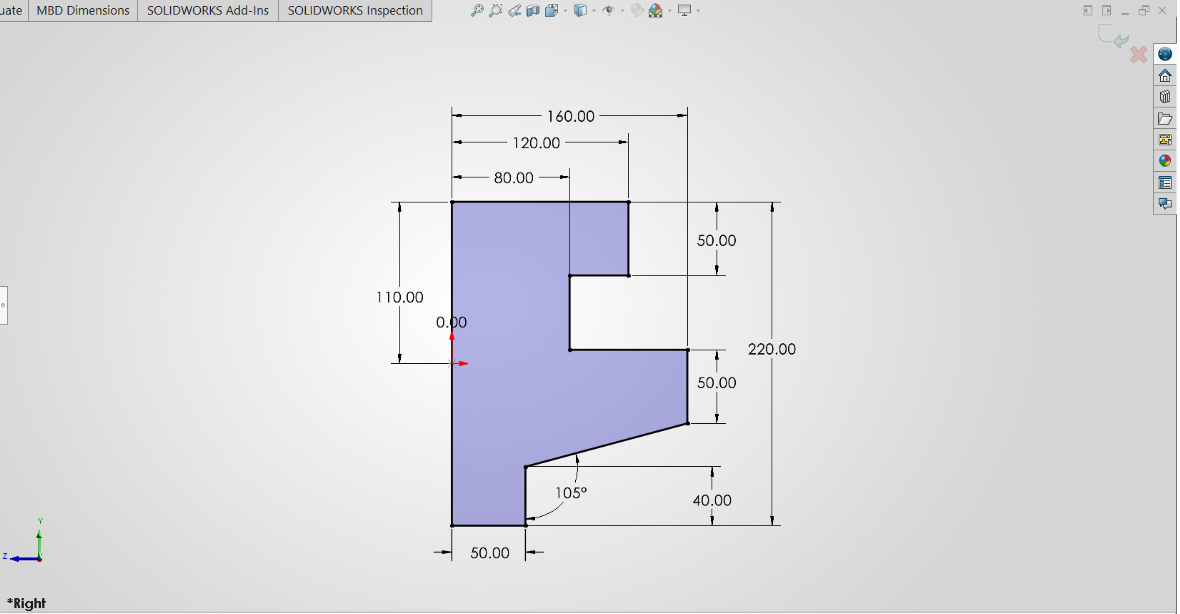
\includegraphics[width=0.7\textwidth]{lab-01/assets/object-5/object-5-snap-1.png}
  \caption{An example of a fully defined 2D sketch.}
  \label{lab_01_fig_sketch_example}
\end{figure}

Once a 2D sketch is created, it can be transformed into a 3D part using various features. One of the most fundamental features is the Extruded Boss/Base. This tool adds depth to a selected sketch profile by projecting it linearly for a specified distance \cite{lab_01_dassault_official}. It is the primary method for creating prismatic parts and adding material based on a 2D shape \cite{lab_01_solidworks_bible}.

\begin{figure}[H]
  \centering
  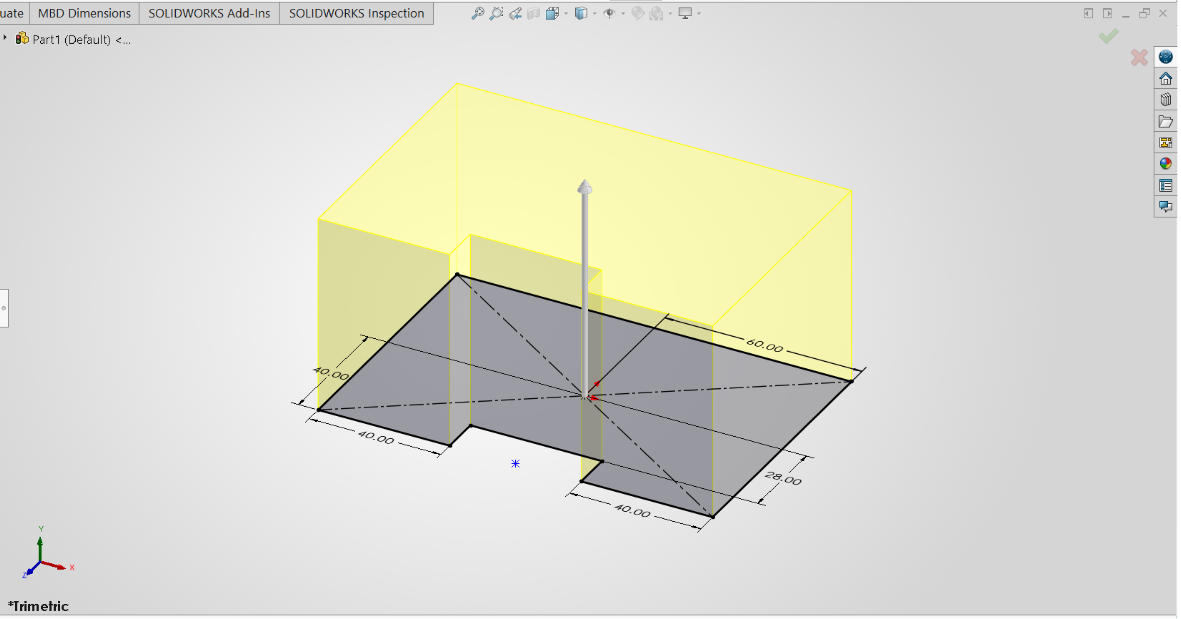
\includegraphics[width=0.7\textwidth]{lab-01/assets/object-4/object-4-snap-2.png}
  \caption{Illustration of the Extruded Boss/Base feature.}
  \label{lab_01_fig_extrude_example}
\end{figure}

Another essential feature for creating cylindrical or axisymmetric parts is the Revolved Boss/Base. This tool creates a 3D model by revolving a 2D sketch around a specified centerline or axis \cite{lab_01_dassault_official}. It is highly efficient for modeling objects like wheels, shafts, and other parts with rotational symmetry. The ability to master both extrusion and revolution provides a powerful toolkit for modeling a vast array of mechanical components \cite{lab_01_cad_fundamentals}.

\begin{figure}[H]
  \centering
  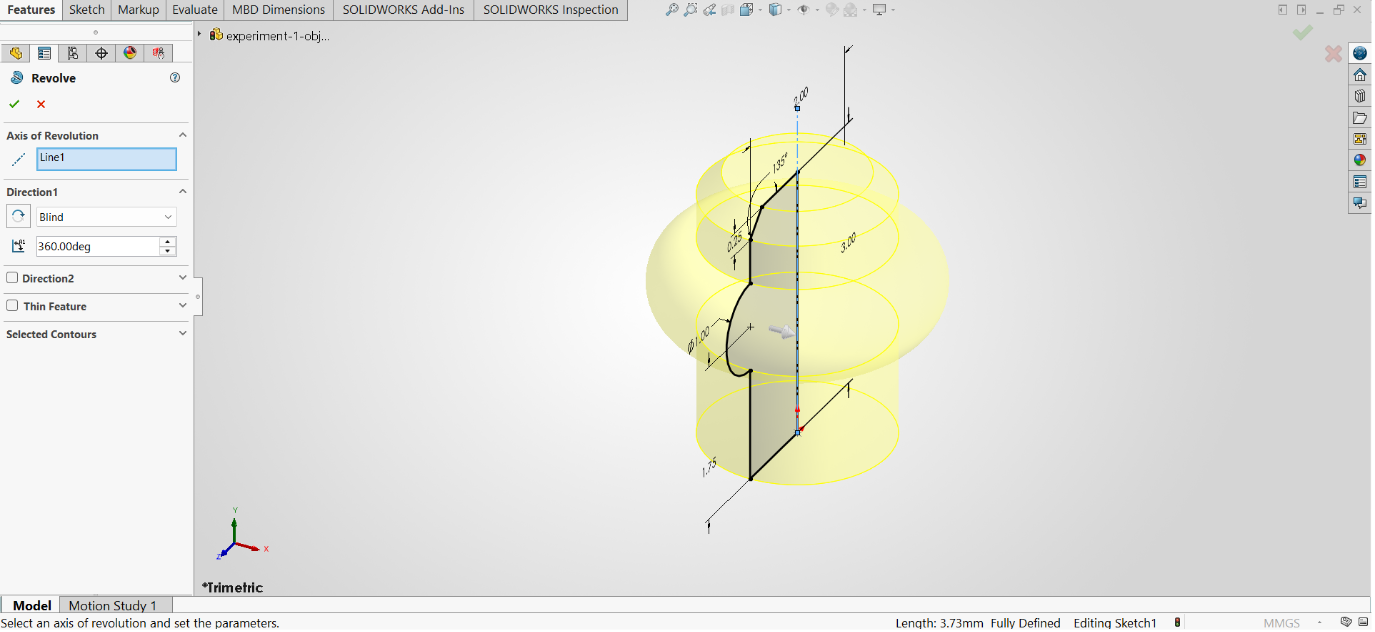
\includegraphics[width=0.7\textwidth]{lab-01/assets/object-10/object-10-snap-2.png}
  \caption{Illustration of the Revolved Boss/Base feature.}
  \label{lab_01_fig_revolve_example}
\end{figure}
